%\documentclass[crop,tikz]{standalone}
%\usepackage{chemfig}
%
%\begin{document}
%
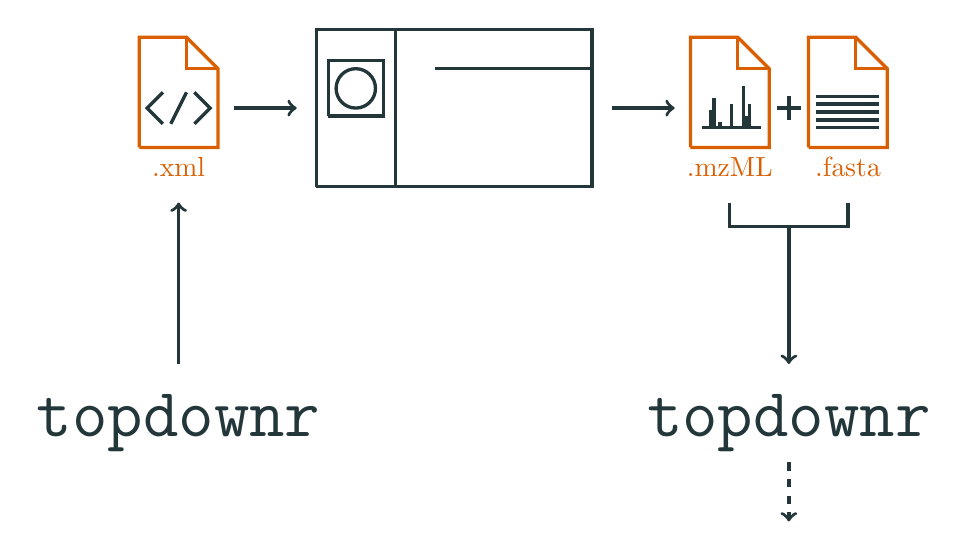
\begin{tikzpicture}

\definecolor{ncolor}{HTML}{1B9E77}
\definecolor{ccolor}{HTML}{D95F02}
\definecolor{bcolor}{HTML}{7570B3}
\definecolor{mcolor}{HTML}{23373B}

\tikzstyle{nline}=[dashed, very thick, color=ncolor]
\tikzstyle{ntext}=[color=ncolor]
\tikzstyle{cline}=[dashed, very thick, color=ccolor]
\tikzstyle{ctext}=[color=ccolor]

\tikzstyle{topdownrtext}=[color=mcolor]
\tikzstyle{massspecline}=[very thick, color=mcolor]
\tikzstyle{arrow}=[very thick, color=mcolor]
\tikzstyle{textcolor}=[color=mcolor]
\tikzstyle{documentline}=[very thick, color=ccolor]
\tikzstyle{documenttext}=[color=ccolor]

\tikzstyle{axis}=[very thick, color=mcolor]
\tikzstyle{peak}=[very thick, color=mcolor]

%\draw[help lines] (0,0) grid (15,10);

\def\doc#1#2#3{
\begin{scope}[shift={#1},scale=#2]
    \draw[documentline] (0, 0) -- (0, 1.4) -- (0.6, 1.4) -- (1, 1) -- (1, 0) -- (0, 0);
    \draw[documentline] (0.6, 1.4) -- (0.6, 1) -- (1, 1);
    \node[documenttext, anchor=north]  at (0.5, 0) {#3};
\end{scope}
}

\def\topdownr#1{
\begin{scope}[shift={#1}]
    \node[topdownrtext, anchor=center] at (0, 0) {\texttt{\Huge{topdownr}}};
\end{scope}
}

\def\massspec#1#2{
\begin{scope}[shift={#1},scale=#2]
    \draw[massspecline] (0, 0) -- (0, 2) -- (3.5, 2) -- (3.5, 0) -- (0, 0);
    \draw[massspecline] (1, 0) -- (1, 2);
    \draw[massspecline] (1, 0) -- (1, 2);
    \draw[massspecline] (1.5, 1.5) -- (3.5, 1.5);
    \draw[massspecline] (0.15, 0.9) -- (0.15, 1.6) -- (0.85, 1.6) -- (0.85, 0.9) -- (0.15, 0.9);
    \draw[massspecline] (0.5, 1.25) circle (0.25);
\end{scope}
}

\def\spectrum#1#2{
\begin{scope}[shift={#1},scale=#2]
% x-axis
\draw[axis] (0,0) -- (10,0);
% peaks
\draw[peak] (1.5,0) -- (1.5,3);
\draw[peak] (2,0) -- (2,5);
\draw[peak] (3,0) -- (3,1);
\draw[peak] (5,0) -- (5,4);
\draw[peak] (7,0) -- (7,7);
\draw[peak] (7.5,0) -- (7.5,2);
\draw[peak] (8,0) -- (8,4);
\end{scope}
}

\def\cross#1{
\begin{scope}[shift={#1}]
    \draw[arrow] (-0.15, 0) -- (0.15, 0);
    \draw[arrow] (0, -0.15) -- (0, 0.15);
\end{scope}
}

\topdownr{(1.5, 2)};
\topdownr{(9.25, 2)};

\doc{(1, 5.5)}{1}{.xml};
    \draw[massspecline] (1.3, 6.2) -- (1.1, 6) -- (1.3, 5.8);
    \draw[massspecline] (1.7, 6.2) -- (1.9, 6) -- (1.7, 5.8);
    \draw[massspecline] (1.6, 6.2) -- (1.4, 5.8);
%\node[textcolor] at (1.5, 6) {\textbf{\textless/\textgreater}};
\massspec{(3.25, 5)}{1};
\doc{(8, 5.5)}{1}{.mzML};
\spectrum{(8.15, 5.75)}{0.075}
\cross{(9.25, 6)}

\doc{(9.5, 5.5)}{1}{.fasta};
\foreach \i in {5.75, 5.85, 5.95, 6.05, 6.15} {
    \draw[massspecline] (9.6, \i) -- (10.4, \i);
};

\draw [arrow, ->] (8.5, 4.8) -- (8.5, 4.5) -- (9.25, 4.5) -- (9.25, 2.75);
\draw [arrow] (10, 4.8) -- (10, 4.5) -- (9.25, 4.5);
\draw [arrow, ->] (1.5, 2.75) -- (1.5, 4.8);
\draw [arrow, ->] (2.2, 6) -- (3.0, 6);
\draw [arrow, ->] (7, 6) -- (7.8, 6);
\draw [arrow, dashed, ->] (9.25, 1.5) -- (9.25, 0.75);

\end{tikzpicture}
%\end{document}
